\chapter{Viewing and evaluating forecasts on a coastal waveguide}
\label{chp:waveguide}
%-----------------------
\begin{quote}
{\small
Originally published as: \texttt{Taylor, A. J. and Brassington, G. B. Sea Level Anomaly Forecasts on a Coastal Waveguide. Weather and Forecasting 35, 757–770 (2020).}

An approach to reduce forecast data to coastal waveguide coordinates is described and demonstrated; informed by the literature on coastally trapped waves (CTW).  All discussion is limited to the Australian mainland but the approach is generally relevant to regions where CTWs influence sea level; including the Americas and Africa. The approach does not produce new forecasts, but aims to focus forecaster attention on aspects of sea level forecasts prominent on the long Australian coast.  The approach also explicitly addresses spatial issues associated with measuring coastal paths. 
Coastal paths are scale-dependent and forecast models discretise the coastal boundary differently. 
A well defined coastal path is required for the quantitative application of CTW concepts such as propagation distance and offshore direction.
The relevance of coastally trapped signals and remote forcing is documented in the oceanographic literature, but is effectively unknown to the general public and rarely mentioned in press reports of sea level events such as nuisance flooding.
Routine presentation of forecast guidance in waveguide coordinates could contribute to the transfer of oceanographic research understanding into forecast narratives.
In addition, the approach can facilitate quantitative forecast evaluations that target CTW properties.
Two ocean forecast systems are contrasted in this framework for the Australian mainland.
One year of daily forecasts are compared, with indications that model baroclinicity is of practical relevance.  
}
\end{quote} 

%--------------------------------------------------------------------------
% introduction
%--------------------------------------------------------------------------
\section{Sea level anomalies and forecast narratives}

Many activities are organised around expectations of coastal water levels over the next few days, including mitigation of  nuisance coastal flooding \citep{Sweet:2014ss, Hague:2019ha}

Still water levels \citep{Pugh:2014di} at the coast are not just a matter of tidal patterns and local storms, but can also be influenced by remote forcing via coastally trapped wave (CTW) mechanisms.
Whilst CTWs have received much academic attention (Section \ref{sec:ctw_background}), it seems the application of the CTW perspective to the evaluation of model guidance and the creation of forecast narratives is routinely absent in the Australian setting. 
This leaves both forecasters and the public with a common assumption that coastal sea level anomalies are driven solely by local weather. Such assumptions may arguably be reinforced by the the manner in which forecasts and evaluation metrics are routinely presented.

Very high impact short scale extreme such as tropical cyclones \citep{McInnes:2016km} are obviously important to coastal decisions but are not the target of this discussion. 


Coastal sea level anomalies are in practice almost always interpreted with reference to conventional tide tables \citep{PCTMSL-sp9}.
Whilst sophisticated sea level decision support systems do exist for some customers \citep{James:2017gj}, in general circumstances the coastal community consult tide tables in light of recently observed anomalies and anomaly trend expectations.
Expectations of how anomalies (or `residuals') may change over the next few days can be based on recent observations, heuristics and numerical forecast guidance \citep{Taylor:2017coa, Horsburgh:2011th}.   Numerical forecasts are the focus of this discussion.
Numerical forecasts of sea level anomaly fields are commonly viewed as topographic maps like Figure \ref{fig:oldcharts}.
%----------------------------
% map guidance
\begin{figure}[!hbt] \centering
    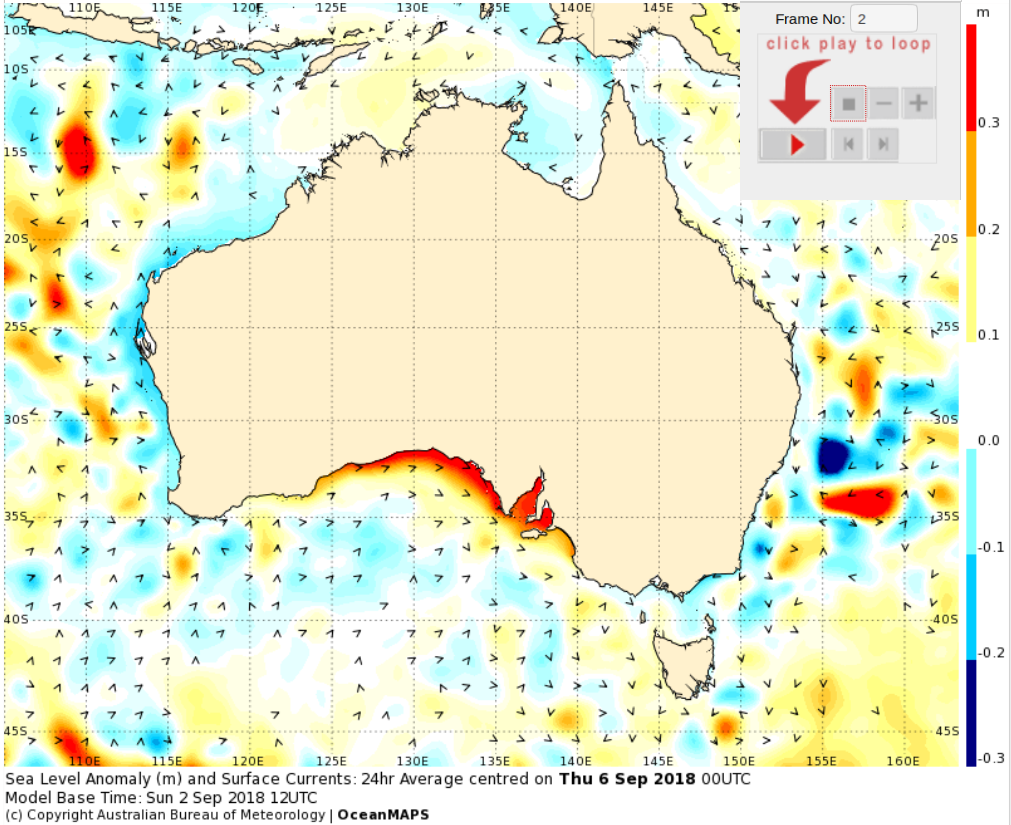
\includegraphics[width=\figwidthBig]{figures/maps/omaps_chart_anim_eg.png}
    \caption{OceanMAPS SLA chart from the Bureau's public website.}
    {Whilst moving patterns are often discernable when animated, these displays do not inherently focus on coastal aspects of the forecast.  \protect\citep{urlBOM_SLA:2018} }
    \label{fig:oldcharts}
\end{figure}  
%----------------------------
Coastal propagation of sea level features can be noticed on animated versions of such maps if the spatial scope is sufficiently large.
But with a wide scope the coastal signal is often visually swamped by the diverse phenomena thus included; such as the eddies shown off the east coast of Australia.
In contrast to the `map' view, consider the propagation-focused phase-space guidance available to tropical weather forecasters \citep{Wheeler:2001} that reduces the many dimensions of a numerical forecast to the propagation of particular patterns around the equatorial wave guide.

Regardless of the forecast guidance source, narrative attribution can be a factor that influences decisions.  
If residents are told that ``...westerly winds push tides from the bay..'' \citep{urlMW:2018}, then they may be perplexed to find their sea gate closed on a windless day.  Public messaging about local strong winds and low pressure are common and useful enough:
``...storm surge is caused when a low atmospheric pressure meteorological system and strong onshore winds force sea levels to rise above normal levels...''
\citep{urlBris:2018}.  But the role of remote winds, wind orientation, persistent and propagating sea level signals seems to be effectively ignored from such descriptions.  


Essentially, we perceive a gap between research understanding and daily forecast narratives.
Routine availability of waveguide views into numerical forecast data may contribute to the transfer of academic understanding to a wider audience and ultimately to improved communications regarding coastal sea level.
Waveguide-based methods to inter-compare heterogeneous forecast data may also facilitate the connection between aspects of the research literature to operational verification and systems development.

We demonstrate one approach for projecting operational ocean forecast data into waveguide coordinates.  Whilst our scope is restricted to the Australian mainland, the concepts may also be relevant to other regions.


%--------------------------------------------------------------------------
% CTW perspective
%--------------------------------------------------------------------------
\section{Coastal waveguide perspective}
\label{sec:ctw_background}

\subsection{Non-operational literature}
The oceanographic literature addressing coastally trapped waves (CTW) is extensive and has prominently featured the Australian mainland. 
The literature has established a common spatial paradigm \citep{Brink:1991dl}  with directions relative to the coast as illustrated in Figure \ref{fig:ctw_typical}. In this context the nomenclature of longshore,alongshore and alongshelf are synonomous. This CTW `natural coordinate' system \citep{gill1982atmosphere} arises from an interest in propagation along a long coastal waveguide. The coordinate schematic indicates an ideal of uniformity long shore and a cross shelf profile that is either flat or deepening monotonically away from a coastal boundary.  
This situation allows for the hybrid of propagation mechanisms involving gravity and potential vorticity, requiring topographic slope, and Rossby adjustment against a coastal boundary.   

%----------------------------
% coord system
\begin{figure}[!hbt] \centering
    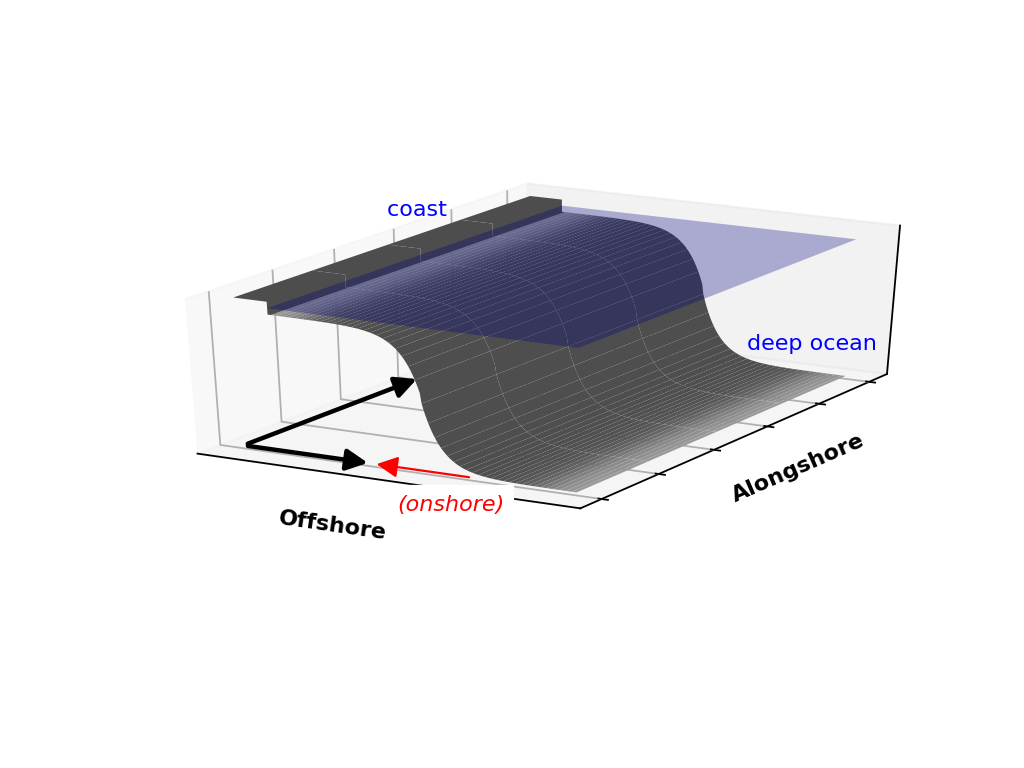
\includegraphics[width=\figwidthFull]{figures/diagrams/ctw_coords.png}
    \caption{Idealised coordinates for coastally trapped waves.}
    {Uniform and large scale in the longshore direction, with a coastal boundary and bathymetry either flat or monotonically increasing offshore. In the southern hemisphere CTWs propagate with the coast on the left. The term CTW covers the range of Kelvin and continental shelf wave mechanisms.  Following \protect\citep{Dale:2001dn}. }
    \label{fig:ctw_typical}
\end{figure}  
%----------------------------
CTW dynamics are generally associated with
sub-inertial frequencies, 
along shelf scales of motion much greater than cross shelf,  
along shelf propagation characteristics
and cross shelf mode decomposition.
Targeted campaigns have demonstrated the relevance of this theory to explaining non-tidal oceanographic observations \citep{Church:1986tl,Merrifield:1992ef,Ding:2012im}.
Coastal trapping also plays an important role in the astronomical tide literature \citep{Anonymous:cyAnLqia}.
The limits of CTW theory have been explored in the literature and these limits are relevant to application at routine weather forecast timescales.
For instance; 
\begin{itemize}
\item energy scattering and leakage \citep{Middleton:1991dq, Merrifield:1994et, Yankovsky:2017en}
\item near inertial and super-inertial frequencies \citep{Dale:2001dn, Dale:1996go} 
\item small scale geometrical irregularities \citep{Wilkin:1990iw,Liao:2011}
\item curvature of along shelf geometry \citep{Grimshaw:1977vu}
\item sensitivity to model choice \citep{Sanson:2012bu}
\item propagating atmospheric features at near resonant speeds \citep{McInnes:2003vl};
\end{itemize}

%-----------------------------------------------
\subsection{How long is the coast and where is it?}
\label{sec:ctw_waveguide}

Applying a CTW perspective to real geography raises the deceptively simple questions of how to measure the length of a propagation path and how to specify along and offshore directions.
Such questions are not problematic for the equatorial waveguide.
But for measuring a waveguide associated with land/sea boundary  raises the well-known `coastline paradox'; by which the length of a statistically fractal feature depends on the measuring scale \citep{Mandelbrot:1967hr} (introduced by L.F.Richardson in another context \citep{Vulpiani2014}).
The literature on CTWs, which inherently involves coastlines, has not directly addressed the statistically fractal character in the attribution of a propagation distance, wind direction or the separation between tide gauges.
Some non-oceanographic literature has however drawn connections in the opposite direction; between the complexity of the Australian coast and marine processes \citep{10.1016/j.margeo.2012.07.011}.

In addition to the non-trivial task of measuring a coast, each discretised model carries its own representation of the coastal interface, often via a binary land/sea mask.
The defacto location of a numerical coast described by a mask can differ noticeably between models even if based on the same foundational bathymetry.
Such differences are especially significant with comparing models configured at different spatial resolutions. 



This situation motivates the application of an algorithmic method to realise a set of model-independent `waveguide' coordinates.
Fundamentally, such an algorithm is a means of defining a coastal path and associated local horizontal directions given a well-defined length scale.
For the present demonstration, a version of the traditional `divider walk' \citep{Xu:1993} algorithm provided a tractable approach to develop a path using the Geospatial Data Abstraction library GDAL \citep{gdal}. 
The path used was based on a relatively high resolution ($\sim$250m) coastline dataset independent from the forecast models themselves.
Figure \ref{fig:mandelbrot_lengths} demonstrates the dependence of waveguide length on divider scale by multiple applications of the algorithm.  The dependence results in an estimate of an effective fractal dimension of $\sim$1.08, comparable to those summarised in \citep{MA2016}.
%----------------------------
% coastline length 
\begin{figure}[!hbt] \centering
    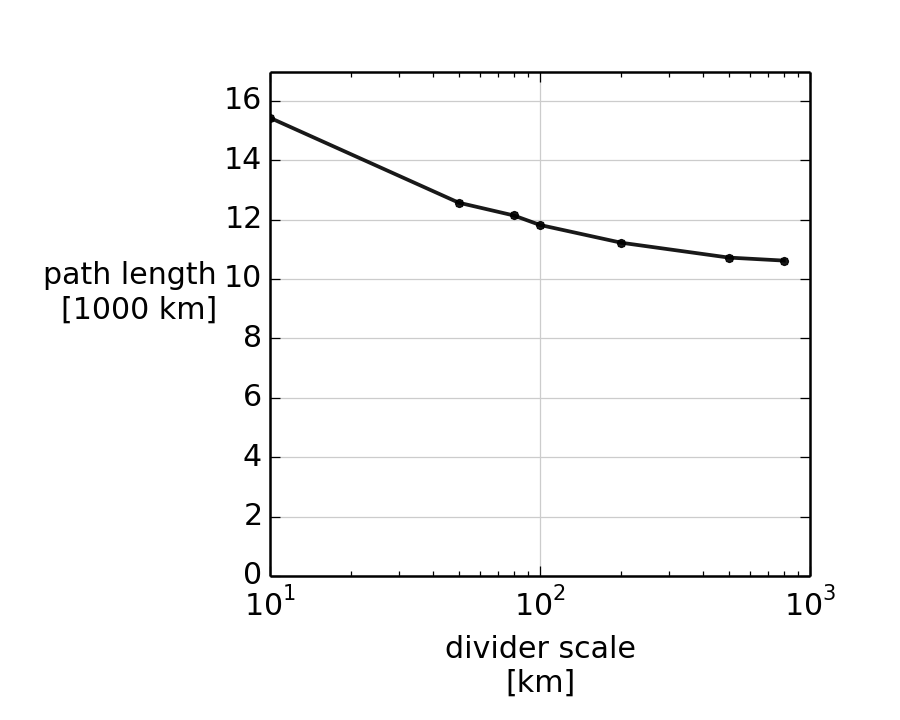
\includegraphics[width=\figwidthBig]{figures/plots/mandelbrot_lengths.png}
    \caption{Waveguide length dependence on scale.}{Total lengths of the Australian waveguide path realised as a function of fixed divider scales, from which an effective fractal dimension of $\sim$1.08 is derived.  
All walk the same anti-cyclonic direction around the coast from an arbitrary start point near Darwin to and end point at Cape York. 
The final divider length in each case is allowed to vary in order to ensure identical start and end points.}
    \label{fig:mandelbrot_lengths}
\end{figure}  
%----------------------------
We emphasise that the idea is to define a longshore length-scale in the realisation of the waveguide path, such that distances and directions have an explicit foundation.
The particular algorithm and scale are not asserted as being unique or optimal and others may present benefits (e.g. the rolling ball method of \citet{Hall:2002bo}).
For this implementation, the length-scale of each divider segment is set proportional to a local Rossby radius of deformation \citep[p.205]{gill1982atmosphere} which is well-defined for the Australian continental path shown.   
This radius depends only on latitude and a wave celerity, which we have configured to match the barotropic mode at a nominal depth of 20m.

This configuration is intended to roughly target the longshore scales associated with CTW generation, but alternative realisations are plainly possible.
The choice of scale primarily impacts the sample directions and derivation of wave speeds from model output - it has no impact whatsoever on the source model's representation of phenomena.
Decomposition of wind vectors into along and offshore directions is closely tied to the details of the path definition.
Sensitivity of the results to the details of path realisation are not explored in this study but will be pursued in future work.      


Figure \ref{fig:CTW_path} shows the waveguide path referenced in subsequent figures.
The shorter lines at each vertex indicate the local offshore direction used to decompose wind vectors and sample coastal cells.
Only the Australian mainland is included with arbitrary start and end points.
Signal expressions around Tasmania or any smaller islands are not addressed. 
%----------------------------
% map waveguide
\begin{figure}[!hbt] \centering
    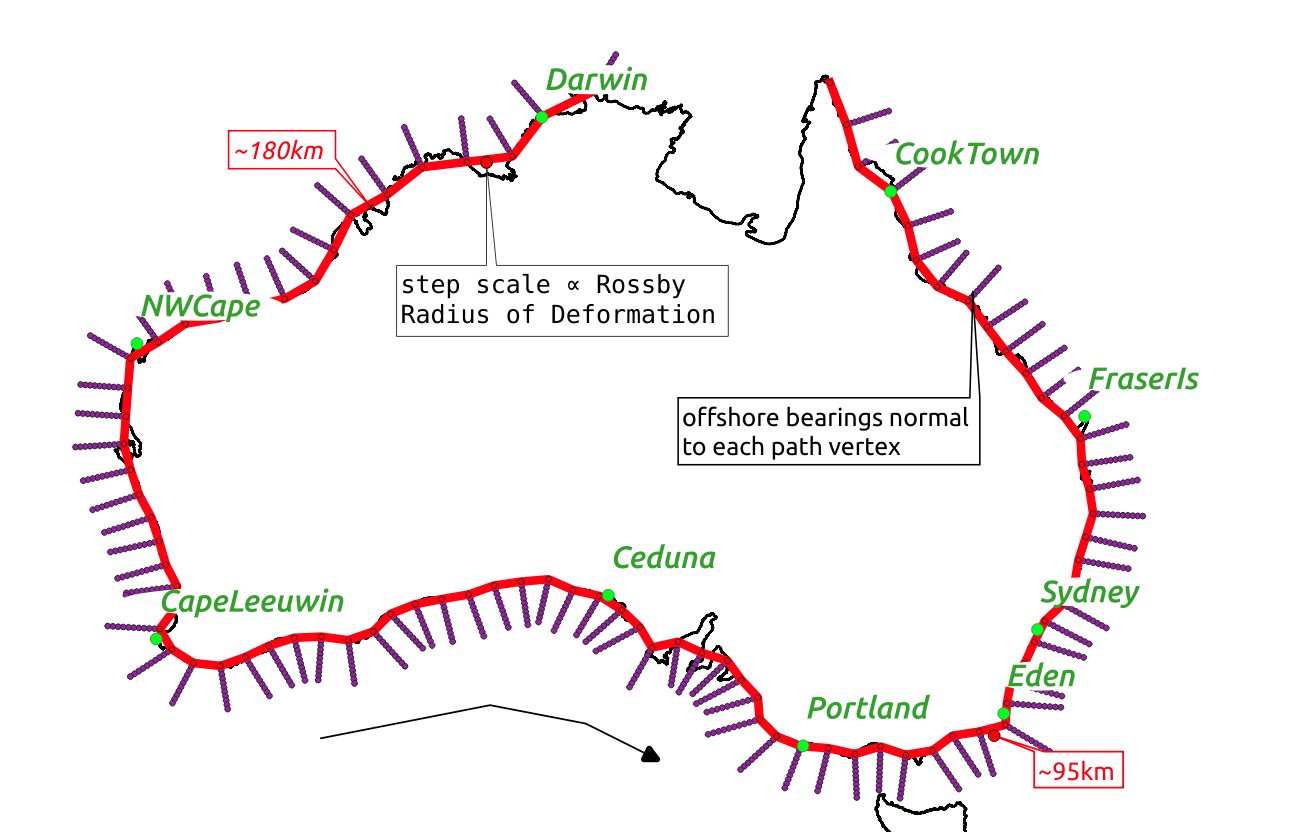
\includegraphics[width=\figwidthFull]{figures/maps/map_overview.png}
    \caption{Coastal waveguide path realisation used for this study.}
    {The path steps around the Australian mainland with anticyclonic direction indicated (southern hemisphere). For this realisation, segment lengths $\protect\propto$ a Rossby Radius of Deformation measure. Across-shore directions (short dark lines) are only locally orthogonal to the path but provide a means to assign a distance coordinate to model samples. The start point is arbitrary and Tasmania is excluded. Locations are named to assist cross-referencing in subsequent figures.}
    \label{fig:CTW_path}
\end{figure}  
%----------------------------

%-------------------------------------------------
\subsection{Projection onto the waveguide path}

The waveguide path is based on an independent high resolution coastline and choice of length scale.
Different data sources were projected onto this path using an algorithmic sampling method.
The sampling method aims to select only grid cells represented as coastal in each model, and to associate locations with the waveguide via orthogonal projection. 
This is effectively a restricted type of `nearest neighbour' sampling with no interpolation between grid points.

For each cross-shore profile line in Figure \ref{fig:CTW_path}, the algorithm essentially looks for the best matching coastal cell by starting out to sea and stepping inwards until the last `wet' cell is found.
Each sample is associated with longshore distance coordinate of the corresponding waveguide vertex.

For tide gauge observations, the inverse process was applied as a geometric projection to assign a waveguide coordinate. 
The projection mapped each tide gauge location to the single closest point on the waveguide following a bearing perpendicular to the matched line segment. 
An arbitrary limit of 50km was applied to limit the spatial extent of the automated projection - which otherwise could match distant island locations to the coastal path. 

To facilitate additional post-processing of the waveguide sampled datasets a two stage linear interpolation process was applied to reduce the data further to a common regular time and space grid for differencing and correlation operations.  

%--------------------------------------------------------------------------
% data
%--------------------------------------------------------------------------
\section{Data sources from the operational centre}

This study originates from the application of a CTW perspective within an operational setting.
Key details of the operational data sources used are outlined below.
Data availability has limited our comparison to the 1-year period from 10-April 2018 to 10-April 2019.

%-----------------------
\subsection{Surface winds and pressure from NWP: ACCESS-G }
\label{sec:access}
Atmospheric forecast inputs were taken from the global numerical weather prediction (NWP) system ACCESS-G \citep{BureauofMeterology:C8IaJ2Qq}.
It is not coupled with any ocean model and employs an observational SST analysis, fixed over each forecast, as a lower boundary condition.
These flux fields are generated on a N512 Gaussian grid with an indicative spatial resolution of $\sim$25km. 

%-----------------------
\subsection{OceanMAPS: data assimilating global ocean circulation}
\label{sec:oceanmaps}
7-day sea level anomaly (SLA) forecasts were taken from the near-global Ocean Model, Analysis and Prediction System (OceanMAPS).
OceanMAPS has now been in operational production for over 10 years across several version upgrades  
\citep{Brassington:2007ut,NMOC:2007wq,BureauofMeterology:2011ta,Brassington:2012wm}.
The dynamic ocean model component of OceanMAPS is based on the Modular Ocean Model (MOM version 4.1) \citep{Griffies:2008vh} configured with a 0.1x0.1 degree regular structured horizontal resolution, hydrostatic free surface, 51 z-levels with 5m top cell, 15m minimum column depth and a split-implicit scheme; where the barotropic calculation is performed at a finer time stepping. 
Atmospheric fluxes from ACCESS-G including surface stress are imposed directly.
Note that barometric pressure and gravitational tidal forces are intentionally \textit{not} applied.

Initial conditions for the ocean state are constrained using an ensemble optimal interpolation data assimilation scheme \citep{Oke:2008wr, sakov:2014}. 
Tide gauge observations are \textit{not} assimilated and are independent.   
Satellite altimeter observations of sea level are assimilated, but not inshore of the shelf break; nominally cut off at the 200m isobath. 
Background error covariances are non-gaussian and based on physical scales resolved by the model.

OceanMAPS produces a new ocean state forecast each day using a multi-cycle ensemble schedule \citep{GaryBBrassington:2013jw}.

Concatenated OceanMAPS data for the period are shown in Figure \ref{fig:hov_eg}. 
%----------------------------
% sla hovmuller
\begin{figure}[!hbt] \centering
    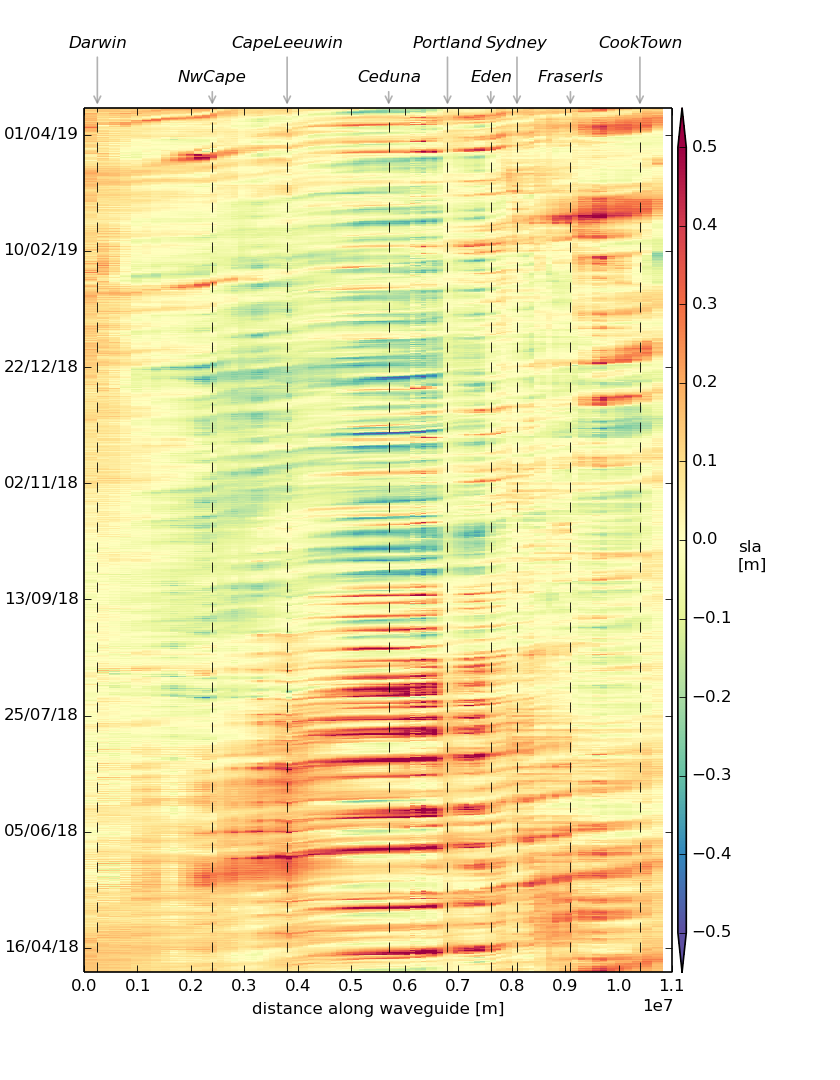
\includegraphics[width=\figwidthFull]{figures/plots/concat_sla_day0_full.png}
    \caption{Concatenated first day of OceanMAPS SLA forecasts.} 
    {Timeseries data for each position have first been centred by removal of the sample mean. Note the distance units are meters and range to $\sim$11000km}
    \label{fig:hov_eg}
\end{figure} 
%----------------------------

%-----------------------
\subsection{Surge: regional depth integrated  }
\label{sec:roms}
Three-day surge forecasts are taken from a national domain 2D configuration of ROMS \citep{Shchepetkin:2005eh} which has been brought into operational production more recently \citep{Allen:2018aa}.  
This operational system produces new forecasts on a 6-hourly warm start cycle with atmospheric forcing from the regional NWP forecasts (ACCESS-R).
No data assimilation is employed and the regional domain is \emph{not} nested in any larger model.
Whilst no baroclinic dynamics are included, the system offers relatively high spatial resolution of $\sim2km$ and alignment with weather forecasts from the more rapidly updated regional NWP system.


For the purposes of this study, a variant of the operational 2D ROMS forecast schedule was run using the identical NWP inputs to the 3D global model, namely ACCESS-G.   
Unlike the operational surge system, barometric pressure fields where not applied to this variant to facilitate direct model inter comparison with OceanMAPS.
Henceforth this system will be referred to as `Surge'.
Whilst this is not strictly operational output, utilising the common NWP source facilitates more meaningful contrast of the ocean model types. 
Modifications beyond the exchange of source NWP were avoided and forecast length was kept at 72 hours.


%-----------------------
\subsection{Adjusted tide gauge observations}
In-situ coastal sea level observations were obtained from a heterogeneous set of real-time tide gauges. 
Many more tide gauges are known to exist within our spatial domain, but we have intentionally used only datastreams available in real-time to Bureau operations.
The resulting spatial sampling of the network is very irregular. 
Coverage along the east coast is most comprehensive.   
The fact that only a subset of these available tide gauges are co-located with barometer instruments influenced the choice to apply a NWP-based inverse barometer adjustment.
This local inverse barometer approximation approach is simplistic \citep{Mathers:2004bk} but pragmatic and formatted as follows:
$ \eta_{LIB} = \frac{ p_{NWP} - p_{ref} }{ \rho g } $
, where reference pressure is fixed at $p_{ref}=101325Pa$, and bulk sea water density is also kept fixed at $1027\frac{kg}{m^3}$. 
Several steps of processing were applied to obtain comparable adjusted residuals.
(1) temporal homogenisation to 1-hour averages (2) subtraction of standard harmonic tide signal (3) adjustment using local inverse barometer approximation based on NWP pressure field.

%--------------------------------------------------------------------------
% comparisons
%--------------------------------------------------------------------------
\section{Viewing operational data in CTW coordinates}

CTWs around the Australian mainland have been recently discussed in the context of general primitive equation ocean models by \citet{Woodham:2013cl} and \citet{Liao:2018jd}; and in the north west of Australia by \citep{Maxime:2019jc}.  The models discussed are closely related to the operational OceanMAPS system. 
In line with the previous literature, these papers address propagation speeds but not how distances between sample locations where measured.
We assert that propagation quantities are rendered more meaningful in this context when the propagation path is made explicit.
The explicit waveguide path approach described in Section \ref{sec:ctw_waveguide} facilitates the generation of new guidance to focus attention on coastal patterns and helps clarify the attribution of propagation quantities.  
Figure \ref{fig:hov_eg} shows a concatenation of the first 24-hours of each OceanMAPS forecast as a familiar `trough-and-ridge' plot \citep{hovmoller:1949}.
Select place names around the Australian mainland are indicated for reference.
Diagonal patterns sloping upward to the right are indicative of signal movement in an anti-cyclonic direction (counter clockwise for the Southern hemisphere).  Both positive and negative signals of this type are evident in many instances.
In contrast, essentially flat (i.e. not propagating) patterns that rise and fall with diurnal frequency are seen in the tropical sections of the domain.   


This projection approach is not limited to a single model or quantity; Figure \ref{fig:collate_g} illustrates an application to several forecast sources sharing a single base date.
A novel aspect of the application to surface winds (a vector quantity) is the decomposition into waveguide-based components - in which the directions are directly related to the length scale specified.
Surface winds are the primary driver of synoptic-scale sea level anomalies and the present inter-comparison is founded on identical atmospheric forcing source being applied to both models. As noted in Section \ref{sec:roms} the 2D surge forecasts are restricted to 3 days.
Broad correspondence of wind stress ($\tau$) and sea level patterns can be seen, especially along the southern shelves as described by \citep{McInnes:2003vl}.
In contrast a relatively regular diurnal pattern is notable in the tropical sections.
%----------------------------
% forecast collection of Hovmullers
\begin{figure}[!hbt] \centering
    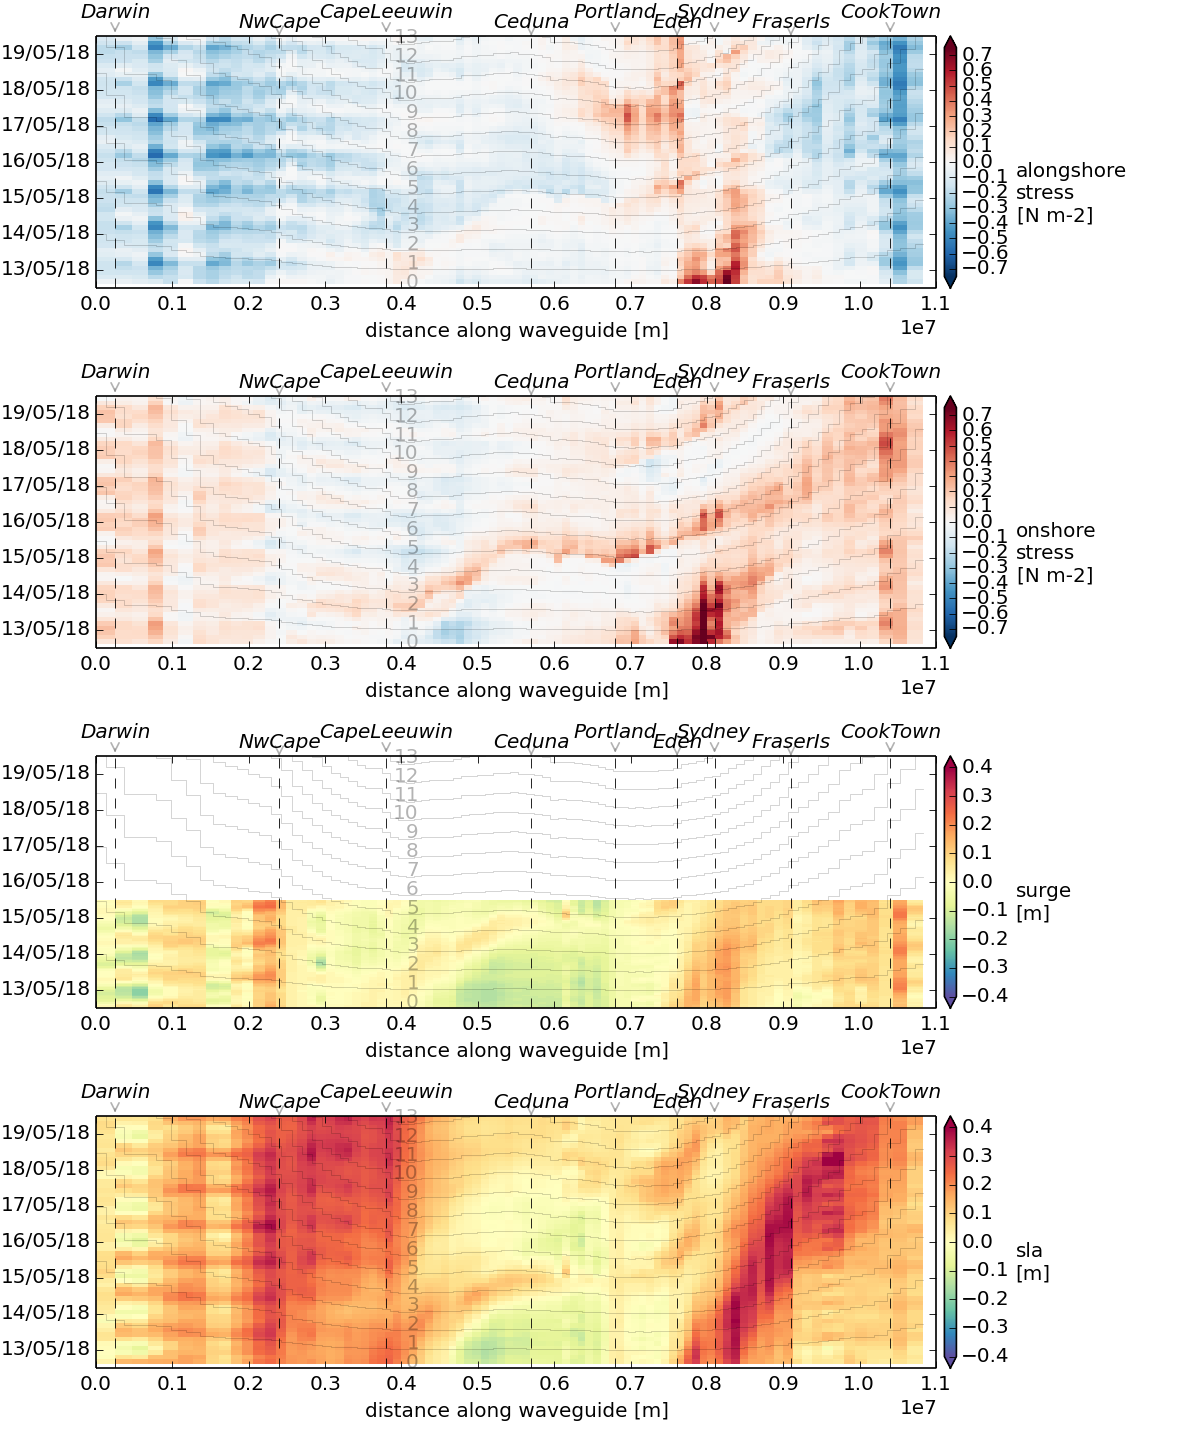
\includegraphics[width=\figwidthFull]{figures/plots/collate_g.png}
    \caption{Single forecast instance visualisation.}
    {Each field is shown on a separate axis with identical time and space limits, feint contours indicate pendulum days to highlight changing inertial periods over the large latitude range. (a) longshore wind stress $\tau_{along}$ units Pa (b) onshore wind stress $\tau_{on}$ units Pa (c) Surge with limited 3-day lead time (d) OceanMAPS.}
    \label{fig:collate_g}
\end{figure}  
%----------------------------
\subsection{Forecast differences viewed in waveguide coordinates}

In addition to providing for focused visualisations, this data reduction method facilitates model inter comparisons that target CTW features.
The following examples contrast behaviour of the barotropic surge model with the lower resolution but dynamically rich global ocean forecasts.
Understanding the limitations of dynamic surge forecasts with regard to CTWs has been recently highlighted as important in the Australian context \citep{Hetzel:2018hh}.   


%-------------------------------
\subsection{Apparent propagation and persistence}
Unlike studies that target the isolation of CTWs \citep{Maiwa:2010tk}, operational users need not distinguish between forced and free propagation as the \emph{apparent} progress of sea level patterns is of primary interest.
Regardless of trapping mechanisms, atmospheric forcing patterns can effectively move around the Australian coast - notably as mid-latitude weather systems travel zonally. 
This movement is reflected by the lagged auto-correlation of wind stress in Figure \ref{fig:Clag0U}.
Apparently anti-cyclonic movement is prominent along the zonally-aligned southern coast but may also occur along non-zonal sections of the coast as patterns of wind alignment progress in time. 
%----------------------------
% correlations
% 0 hours
\begin{figure}[!hbt] \centering
    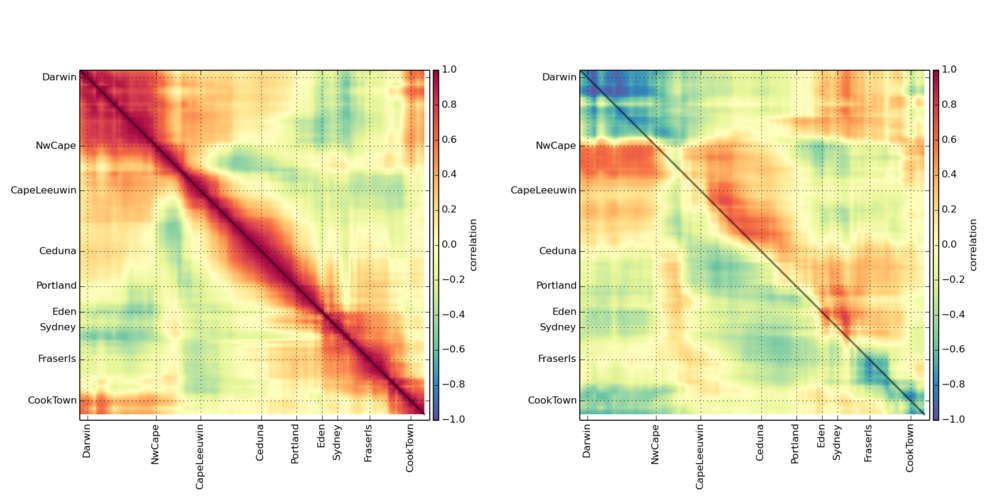
\includegraphics[width=\figwidthFull]{figures/plots/concatC_U_gstr_lag_000.png}
    \caption{Cross-correlation at lag of zero hours for $\tau_{along}$.}
    {$\tau_{along}$ lagging (a) $\tau_{along}$ (b) $\tau_{on}$}
    \label{fig:Clag0U}
\end{figure}
%----------------------------
We suggest that a forecast like that shown in Figure \ref{fig:collate_g} may be helpfully narrated as ``a pattern of sea level anomalies moving along the southern mainland and up the NSW coast over the next 7 days'' without any reference to CTWs or physical processes.
Whilst attribution to can aid forecaster interpretation, it is not the primary concern of public narratives.   
 
Inspection of Figure \ref{fig:hov_eg} shows visually coherent structures from which apparent propagation speeds can be derived, corroborating the $\sim$3.4m/s speeds described by \citet{Woodham:2013cl} and others along the east coast.
Though without temporal filtering, faster features more indicative of Kelvin waves ($\sim$25m/s) are also present.   
An implication of Figure \ref{fig:mandelbrot_lengths} is that such speed estimates are dependent on the length scale used to measure the coastal path. 

%-------------------------------
\subsection{Wind stress orientation and correlation}
Whilst sub-inertial CTW theory is formulated only in terms of longshore winds, the onshore component is also a factor in sea level forecasts \citep{Tilburg:2004cg}.
Propagation of signal along the waveguide means that non-local winds can also be important; a fact that we assert is not commonly appreciated by forecasters or the general public. 


Lagged cross-correlations between the datasets projected into waveguide coordinates are relatively simple given that the data are reduced to a common 1D spatial path. 
Some of the structure in these correlations simply reflect details of interpolation and spatial sampling, but meaningful interpretation is still possible; recalling that the same atmospheric forcing is apply to both models.


At zero lag, Figure \ref{fig:Clag0U} provides some indication of typical length scales of the forcing weather systems.  
The peculiar decomposition into longshore and cross-shore directions (wind stress $\tau_{along}$ and $\tau_{on}$) imposed by the geometry of this path realisation is also apparent, with much shorter scales at coastal 'corners' such as Cape Leeuwin.  
Correlations between wind components and modelled sea level at a lag of nearly 3-days are shown in Figures \ref{fig:Clag66sla} and \ref{fig:Clag66surge}.  
Spatially coherent correlation peaks offset to the right of the main diagonal in these figures are interpreted as systematic anti-cyclonic signal propagation. 
Contrasts between the models are evident on the east coast north of Sydney that may reflect the role baroclinic modes.
%-------------------------------------------
% 66 hours
\newcommand\CAPTIONb{Cross-correlation at lag of 66 hours}
\begin{figure}[!hbt] \centering
    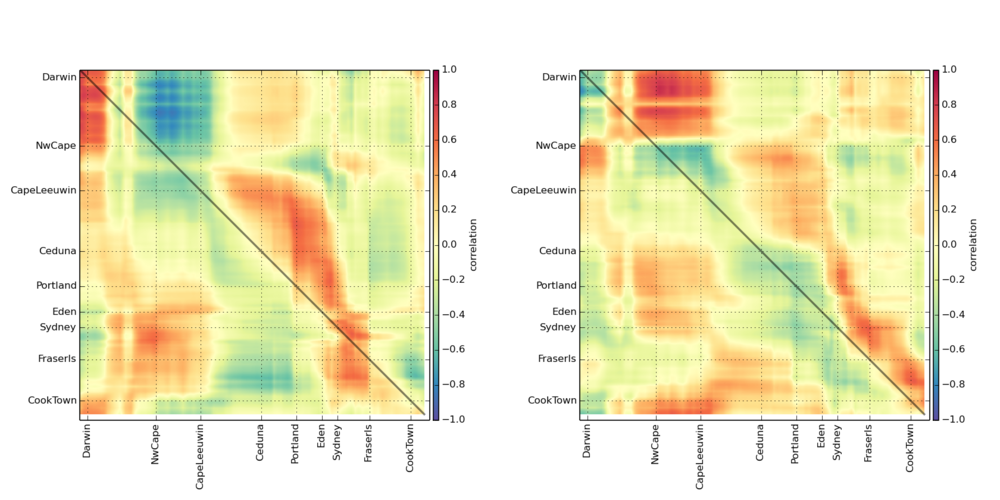
\includegraphics[width=\figwidthFull]{figures/plots/concatC_sla_lag_066.png}
    \caption{\CAPTIONb{} for OceanMAPS}
    {OceanMAPS response lagging (a) $\tau_{along}$ (b) $\tau_{on}$} 
    \label{fig:Clag66sla}
\end{figure}

\begin{figure}[!hbt] \centering
    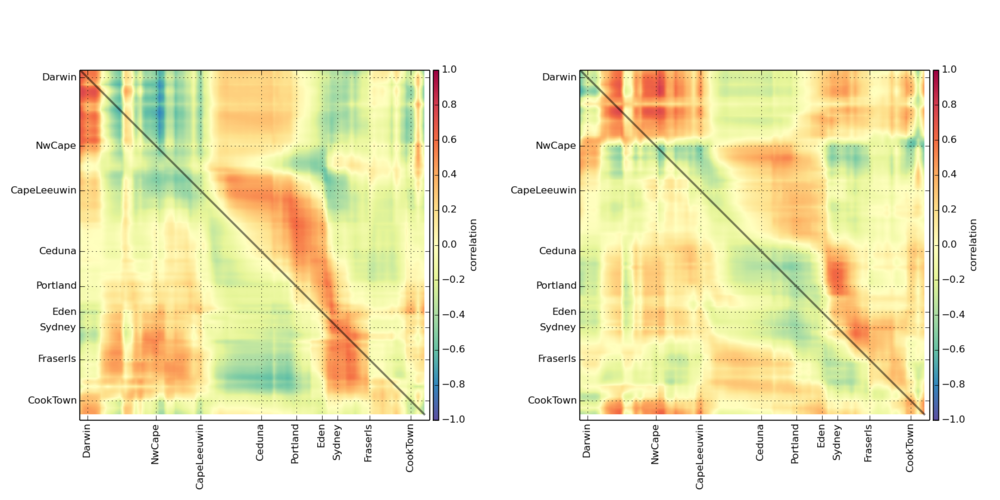
\includegraphics[width=\figwidthFull]{figures/plots/concatC_surgeg_lag_066.png}
    \caption{\CAPTIONb{} for Surge}
    {Surge response lagging (a) $\tau_{along}$ (b) $\tau_{on}$} 
    \label{fig:Clag66surge}
\end{figure}
%-------------------------------------------


%-------------------------------
\subsection{Baroclinicity and shelf resolution}
Differences between the interpolated tide observations, OceanMAPS and Surge forecasts are shown in Figures \ref{fig:diff_tide_omaps} and \ref{fig:diff_tide_surge} respectively.
%----------------------------
% differences
\newcommand\CAPTIONc{SLA differences from concatenated datasets}
\begin{figure}[!hbt] \centering
    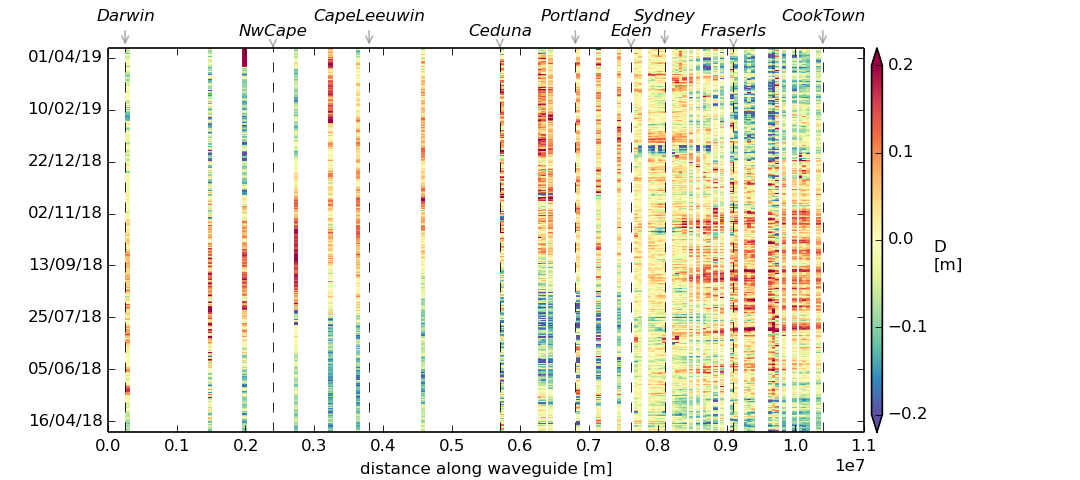
\includegraphics[width=\figwidthFull]{figures/plots/interpTdiff_obs_sla_day0_d0.png}
    \caption{SLA differences - Tide gauges versus OceanMAPS.}
    \label{fig:diff_tide_omaps}
\end{figure}

\begin{figure}[!hbt] \centering
    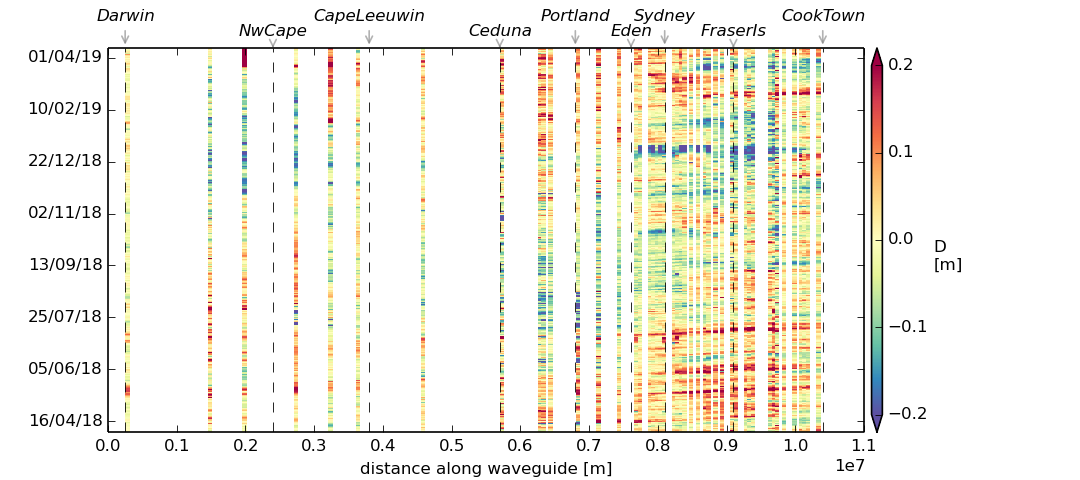
\includegraphics[width=\figwidthFull]{figures/plots/interpTdiff_obs_surgeg_day0_d0.png}
    \label{fig:diff_tide_surge}
\end{figure}

\begin{figure}[!hbt] \centering
    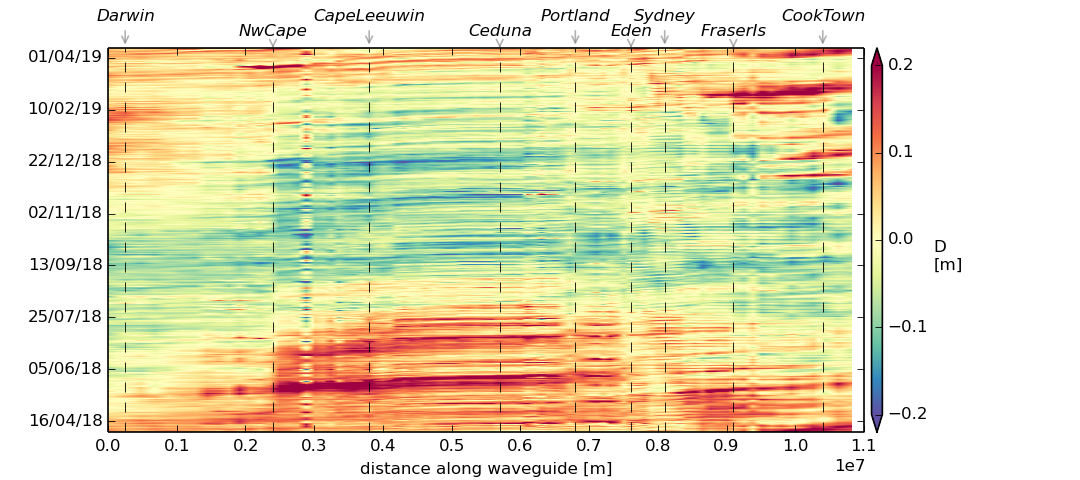
\includegraphics[width=\figwidthFull]{figures/plots/interpRdiff_sla_surgeg_day0.png}
    \caption{SLA differences - OceanMAPS versus Surge.}
    {Patterns of anticyclonic propagation are apparent and indicative of systemic differences in representation between the models. These features are set against the slower seasonal patterns of difference.}
    \label{fig:diff_omaps_surge}
\end{figure}
%----------------------------
The relative spatial density of available tide gauge data along the east coast is prominent.
Differences between the two models are shown in Figure \ref{fig:diff_omaps_surge}. 
Many of the differences are again simply issues of spatial sampling, especially for the Surge model around the bays near North West Cape.
However structured patterns of difference will at least partially reflect systematic deficiencies in each model.

The relatively large difference between the two forecasts may reflect the lack of baroclinicity in the Surge model.
Dynamics relevant to some forms of CTW propagation are excluded from an ocean model without any buoyancy stratification.   
Apparently propagating patterns of additional signal are present in the OceanMAPS forecasts starting from around Cape Leeuwin.
For instance, the feature on the east coast in mid-May has an apparent celerity of $\sim$3.4m/s; consistent with CTW features reported by \citet{Woodham:2013cl}.


\citet[p.312]{Liao:2018jd} specifically comment that ``...data from the OFAM reanalysis in \citet{Woodham:2013cl} were based on a horizontal resolution of 10km which was not high enough for the Australian east coast ...[and] vertical resolution [details] ... could lead to further inaccuracy in ...CTW amplitude calculation[s].''.
Despite this coarse representation of the narrow east coast shelf, the fact that CTW-like features appear in the OceanMAPS sea level signal, but not in the higher resolution Surge forecasts is interesting and possibly reflects an advantage in allowing at least some representation of baroclinic modes.   
Figure \ref{fig:skill_mebs} summarises and contrasts the SLA forecast skill of the two systems for categorised lead times of 0-24 hours (day-0), 24-48 hour (day-1) and 48-72 hours (day-2).  Day-0 difference data is that shown in Figures \ref{fig:diff_tide_omaps} and \ref{fig:diff_tide_surge}.
On this measure, OceanMAPS notably out-performs the Surge forecast along the east coast from Eden to Fraser Island.
%----------------------------
\begin{figure}[!hbt] \centering
    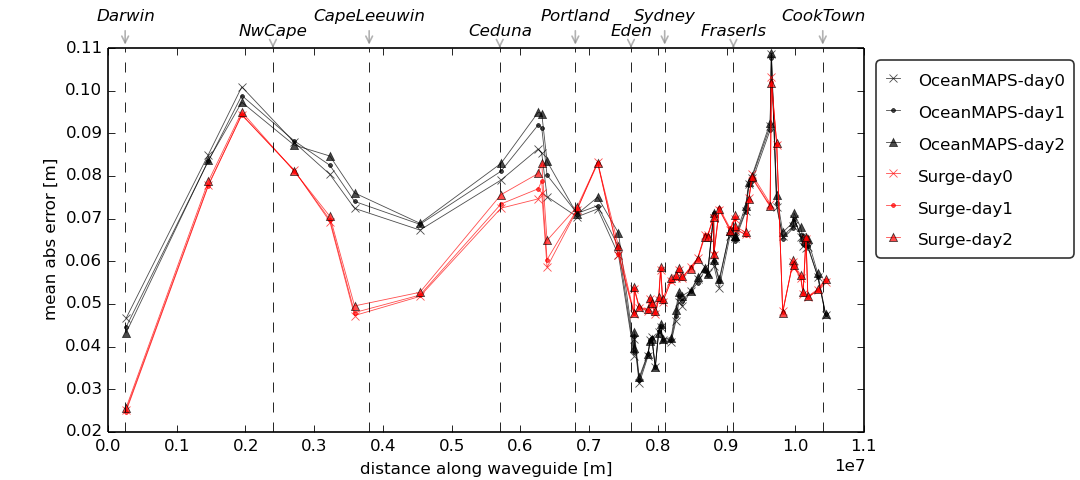
\includegraphics[width=\figwidthFull]{figures/plots/plot_skill_path_mebs.png}
    \caption{Forecast skill along the waveguide.}
    {Mean absolute error for SLA at tide gauge locations. Forecasts are categorised into lead times of 0-24 hours (day-0), 24-48 hours (day-1) and 48-72 hours (day-2). Lower error indicates better overall skill for the 1 year period. OceanMAPS outperforms Surge along the populated east coast. Forecast skill decay with lead time is evident in both models - except for the apparent unusual inversion in the north west.}
    \label{fig:skill_mebs}
\end{figure}
%----------------------------
As this section of the Australian coast is characterised by such a narrow continental shelf, better skill results from the model with lower horizontal resolution is at face-value surprising.  But when this skill is viewed in light of a CTW perspective, it points to the east coast being a region where  propagating sea level signals are significant and where representing baroclinicity provides a tangible advantage to the forecast model.

%--------------------------------------------------------------------------
% Discussion
%--------------------------------------------------------------------------
\section{Chapter discussion}
We assert that a waveguide perspective can provide complimentary insight into the interpretation of daily sea level forecasts and assist in promoting the transfer of research understandings to daily operations.  
Whilst the Australian coastline has been the sole focus of this study, the approach taken could also apply to similar long coastlines, including the Americas and Africa. Whether forecast narratives in those regions also under-play remotely forced coastal sea level is beyond our scope, but a waveguide perspective may offer some insight into explaining the \citet{DiLiberto:2011dya} finding that a 5-day bias correction improved forecasts skill for particular depth-integrated surge models in a North American context.


The way that numerical forecast guidance is framed informs the forecast narratives that can ultimately influence decisions made at the coast.
Given the apparently common over-emphasis on the role of local weather effects on coastal sea level anomalies, a CTW perspective onto sea level forecasts may help direct attention to the relevance of broader longshore patterns and remote winds.
Such a perspective could inform narratives without the need for reference to potentially obfuscating academic terms, for example:
``
...a pattern of sea level anomalies moving up the NSW coast over the next 3 days will raise sea levels... 
''

Beyond the application to daily forecasts, the approach presented will facilitate forecast evaluations that target coastal propagation.
Coastal propagation characteristics are rendered more directly compariable by the reduction of heterogeneous gridded data onto a well-defined 1D waveguide. 
Whilst it is common practice to approach surge forecasting with depth-integrated ocean models, especially in the context of tropical cyclones \citep{Veeramony:2017}, the abilty of models to represent CTWs could have implications for Australian system development priorities. 
Pursuing the work of \citet{Hetzel:2018hh} regarding the (in)adequacy of barotropic ocean models is of particular relevance to the Australian context where the trade-off between representing baroclinic dynamics, spatial resolution and uncertainty is of practical importance.  
     

Improved methods to develop the idea of waveguide coordinates are surely possible.
Sensitivity of the results to waveguide path realisation should be explored and potentially leveraged for specific outcomes.
For instance, to define a coastline that highlights wind orientations of particular significance to driving sea level; extending the manner in which \citet{Tilburg:2004cg} relates measured winds to measured sea level to derive a parametric anomaly forecast model. 


Extension of the 1D approach to also sample model fields along cross-shore profiles (not just at coastal points) could offer insight into the representation of relevant dynamics.
But the algorithm presented is unlikely to be suited to such an extension as it does not provide a conformal map.  Whilst the coordinate directions are orthogonal at the coast, the directions loss meaning with distance offshore to the extent that the profiles can intersect.
  


Well-defined CTW coordinates could in principle facilitate the introduction of process specific numerical models like that of \citet{Brink:1987va} employed by \citet{Liao:2018jd} into the operational setting.
Accurate representation of certain ocean current features in particular could motivate this. 
However, a process-targeted model direction is at odds with the ongoing evolution of increasingly `concrete' generalised simulations \citep{Petersen:2012tr} that are the mainstay of operational forecast centres, so the benefits of a dedicated CTW system would require extraordinary justification.

Forecasts at the coastal interface are both important and challenging. Evaluation approaches that isolate this domain can help align skill metrics with user significance.  
Although not pursued in this discussion, projection of candidate forecast system onto a common wave-guide path will allow for detailed quantitative comparisons of propagation characteristics.  Various signal processing techniques are available to exploit spatially-ordered sets of timeseries data for propagation analysis; though the limitations of complex empirical orthogonal functions described by \citet{Merrifield:1990um} should serve as a general caution about over-interpretation.   


%\subsection{ Application to new ESM forecast suites}
% access-s TBC


Finally we note that whilst forecasting systems will continue to be updated and extended, the data projection and presentation approaches demonstrated here are model-independent and potentially employed as a generic capability within forecaster visual interface.




